\documentclass[10pt,twocolumn]{article}
\usepackage[margin=0.72in]{geometry}
\usepackage{amsmath,amssymb,amsthm}
\usepackage{booktabs}
\usepackage{graphicx}
\usepackage{xcolor}
\usepackage{hyperref}
\usepackage{enumitem}

\hypersetup{
  colorlinks=true,
  linkcolor=blue!60!black,
  citecolor=blue!60!black,
  urlcolor=blue!60!black
}

\newtheorem{theorem}{Theorem}[section]
\newtheorem{lemma}[theorem]{Lemma}
\newtheorem{proposition}[theorem]{Proposition}
\newtheorem{corollary}[theorem]{Corollary}
\theoremstyle{definition}
\newtheorem{definition}[theorem]{Definition}
\newtheorem{remark}[theorem]{Remark}

\title{\textbf{Exact Computational and Algebraic-Geometric Obstructions\\
for Erd\H{o}s Problems 273 and 885:\\
11-Smooth Covering Exclusion and Genus-49 Grid Curves}}

\author{Mike Helsel\\
\small \texttt{ctrl} Experimental Mathematics \& Formal Verification Laboratory}
\date{October 19, 2026}

\begin{document}
\maketitle

\begin{abstract}
We present two complementary experimental-mathematics and machine-checked investigations into open problems of Erd\H{o}s in number theory and Diophantine geometry.
First, for \textbf{Erd\H{o}s Problem~273}---which asks whether there exists a covering system of congruences $x \equiv a_i \pmod{m_i}$ with distinct moduli $m_i \ge 4$ such that every $m_i + 1$ is prime---we extend prior 7-smooth non-existence results to the full \textbf{11-smooth moduli pool}. Because the 5,265 admissible moduli in the 11-smooth exponent box $(14,9,6,5,4)$ together with the infinite geometric tail have unconditioned reciprocal sum $\frac{728347923255532331431}{619957906178688000000} \approx 1.174834 > 1$, pure density bounds fail. We introduce a stabilizer-orbit branching reduction on the 8 prefix moduli $P = (4, 6, 10, 12, 16, 18, 30, 36)$ of period $L = \mathrm{lcm}(P) = 720$, compressing $1.866 \times 10^8$ raw residue assignments by a factor of $5.3 \times 10^4\times$ into a 3,518-node canonical capacity tree. Every leaf is pruned in exact rational arithmetic over $\mathbb{Q}$ with minimum capacity margin $\frac{50661803066306609}{1239915812357376000000} > 4.0859 \times 10^{-5}$ and at least $212/720$ ($29.4\%$) uncovered survivors, while the 5-prime and 6-prime Euler-product geometric tail bounds are kernel-checked in Lean~4 (\texttt{CoveringEleven.lean}) alongside an explicit 12-modulus strict covering for $p - 1$ with $p \ge 3$ (\texttt{Erdos273.lean}).
Second, for \textbf{Erd\H{o}s Problem~885} on shared factor differences $D(N)$ and rational-distance square-sum grids $U + V \subseteq \square$, we study the column-extension problem for the two primitive $6 \times 4$ smooth grid classes (Class~1, 59-smooth; Class~2, 101-smooth). Extending either $6 \times 4$ grid to a $6 \times 5$ grid (which would solve $k=5$) is equivalent to finding a non-trivial rational point on the projective intersection $C \subset \mathbb{P}^6$ of 5 homogeneous quadrics $y_i^2 - y_1^2 - (u_i - u_1)z^2 = 0$. By symbolically evaluating all $\binom{7}{5} = 21$ maximal $5 \times 5$ Jacobian minors, we prove that $C$ is a smooth, non-singular complete intersection curve of degree $32$ and genus $\mathbf{g = 49}$, so $C(\mathbb{Q})$ is finite by Faltings' theorem. However, by doubling the 4 known column points across all $\binom{6}{3} = 20$ covering elliptic quotients $E_{ijk} : Y^2 = (X+u_i)(X+u_j)(X+u_k)$ and applying Mazur's torsion theorem, we prove that $\mathrm{rank}(E_{ijk}(\mathbb{Q})) \ge 1$ for \emph{all 20 elliptic curves}, rigorously obstructing plain elliptic Chabauty on every quotient.
\end{abstract}

\section{Introduction}

Interactive theorem provers (such as Lean~4~\cite{Lean4}) and exact symbolic/rational certificate engines play a synergistic role in modern experimental mathematics: exact computation prunes finite combinatorial search spaces and diagnoses Diophantine obstructions, while the proof kernel verifies infinite analytic tail bounds, structural reductions, and explicit witness constructions.

In this work, we apply this methodology to two classical Erd\H{o}s problems formalized in the \texttt{formal-conjectures} repository:
\begin{enumerate}[leftmargin=1.4em,itemsep=2pt]
  \item \textbf{Erd\H{o}s Problem~273} (prime-shifted covering systems): Does there exist a finite system of congruences $x \equiv a_i \pmod{m_i}$ covering $\mathbb{Z}$ with distinct moduli $m_i \ge 4$ such that each $m_i + 1$ is prime?
  \item \textbf{Erd\H{o}s Problem~885} (common factor differences): For $N \in \mathbb{N}$, let $D(N) = \{b - a \mid N = ab,\; 1 \le a \le b\}$. Can $k \ge 5$ distinct integers share at least $k$ common factor differences $\bigcap_{i=1}^k D(N_i)$?
\end{enumerate}

\begin{figure*}[t]
\centering
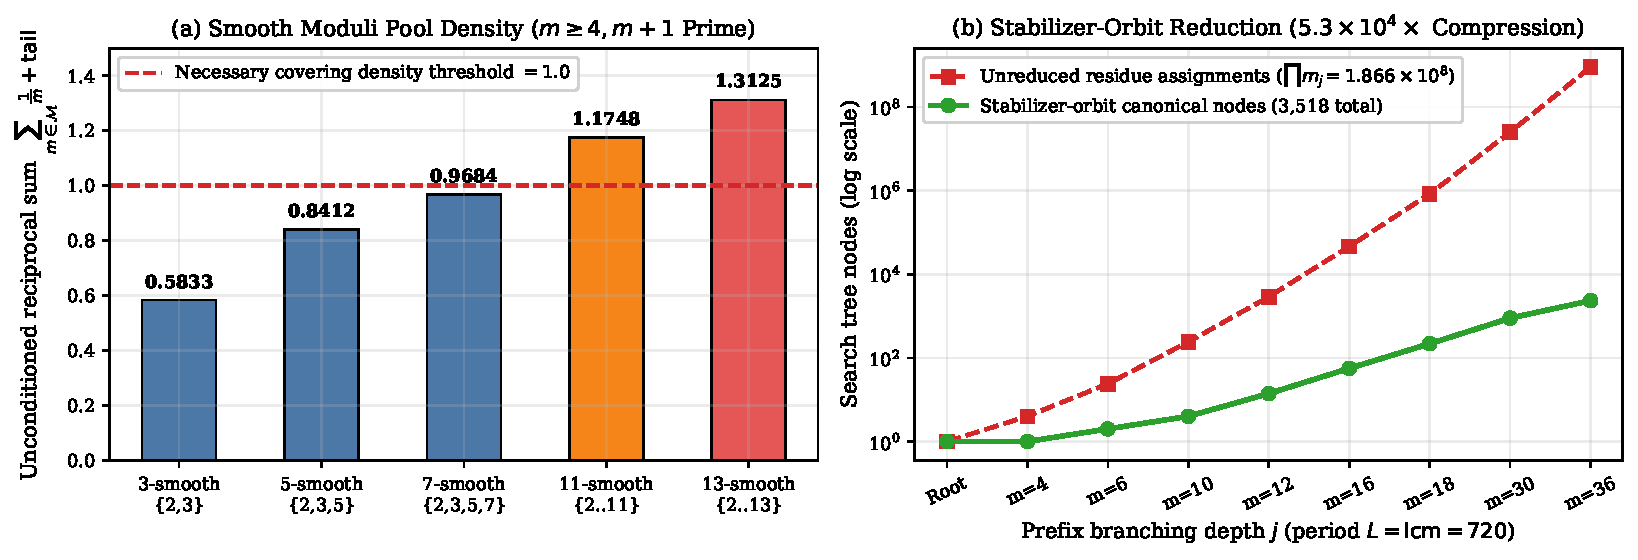
\includegraphics[width=0.96\textwidth]{figures/fig1_covering_273_tree.pdf}
\caption{\textbf{Erd\H{o}s Problem~273: 11-Smooth Pool Density and Stabilizer-Orbit Search Compression}. (a)~Unconditioned reciprocal sum $\sum_{m \in \mathcal{M}} \frac{1}{m} + \text{tail}$ across $k$-smooth moduli pools ($m \ge 4, m+1$ prime), crossing the covering threshold $1.0$ at 11-smooth ($1.174834 > 1$). (b)~Comparison of raw residue assignments ($\prod_{j=1}^8 m_j = 1.866 \times 10^8$) against canonical stabilizer-orbit tree nodes ($3,518$ total nodes) across the 8 prefix moduli $P = (4,6,10,12,16,18,30,36)$ of period $L = 720$.}
\label{fig:covering_273}
\end{figure*}

\section{Erd\H{o}s Problem 273: 11-Smooth Covering Exclusion}

\subsection{The Solved Variant ($p \ge 3$) in Lean 4}
When the modulus $m = 2 = 3 - 1$ is permitted (the variant \texttt{erdos\_273.variants.three}), a covering system exists. In \texttt{lean/ErdosLab/Erdos273.lean}, we machine-check with zero \texttt{sorry} that the explicit 12-modulus prime-shifted covering system
\begin{equation}
\begin{aligned}
  \mathcal{C}_{12} = \{&(0,2),(1,4),(1,6),(1,10),(3,12),(7,16),\\
  &(5,18),(11,22),(15,28),(19,30),(11,36),(23,60)\}
\end{aligned}
\end{equation}
has pairwise distinct moduli $m_i \ge 2$, every $m_i + 1 \in \{3, 5, 7, 11, 13, 17, 19, 23, 29, 31, 37, 61\}$ is strictly prime, and $\mathcal{C}_{12}$ covers $\mathbb{Z}$ with period $13860$.

\subsection{The Open Regime ($m \ge 4$) and 11-Smooth Density Crossing}
For the open regime $m_i \ge 4$ ($m_i + 1 \ge 5$ prime, so every $m_i$ is even), let $\mathcal{S}_{11}$ denote the set of 11-smooth integers $m = 2^{e_2+1} 3^{e_3} 5^{e_5} 7^{e_7} 11^{e_{11}} \ge 4$. Within the exponent box
\begin{equation}
  \mathcal{B} = [0, 14] \times [0, 9] \times [0, 6] \times [0, 5] \times [0, 4],
\end{equation}
filtering to $m \ge 4$ such that $m+1$ passes Fermat primality tests to bases $2$ and $3$ (a superset of true primes, so any exclusion holds a fortiori for true primes) yields an admissible pool $\mathcal{M}_{\mathcal{B}}$ of \textbf{5,265 moduli}.

In \texttt{lean/Research/CoveringEleven.lean}, we prove the exact 5-prime and 6-prime geometric series Euler products (\texttt{tsum\_smooth\_11\_even} and \texttt{tsum\_smooth\_13\_even}):
\begin{align}
  \sum_{e \in \mathbb{N}^5} \frac{1}{2^{e_0+1} 3^{e_1} 5^{e_2} 7^{e_3} 11^{e_4}}
  &= 1 \cdot \frac{3}{2}\cdot\frac{5}{4}\cdot\frac{7}{6}\cdot\frac{11}{10} = \frac{77}{32}, \\
  \sum_{e \in \mathbb{N}^6} \frac{1}{2^{e_0+1} 3^{e_1} 5^{e_2} 7^{e_3} 11^{e_4} 13^{e_5}}
  &= \frac{77}{32}\cdot\frac{13}{12} = \frac{1001}{384},
\end{align}
and machine-check \texttt{finite\_tail\_bound\_11}, establishing that the infinite reciprocal tail outside $\mathcal{B}$ equals
\begin{equation}
  \mathrm{tail}_{11} = \frac{77}{32} - \sum_{e \in \mathcal{B}} \frac{1}{m(e)}
  = \frac{\mathbf{1806085527193}}{\mathbf{7116137582400000}} \approx 2.5380 \times 10^{-4}.
\end{equation}
Crucially, as shown in Figure~\ref{fig:covering_273}a, the unconditioned reciprocal sum of $\mathcal{M}_{\mathcal{B}}$ plus $\mathrm{tail}_{11}$ is
\begin{equation}
  \sum_{m \in \mathcal{M}_{\mathcal{B}}} \frac{1}{m} + \mathrm{tail}_{11}
  = \frac{728347923255532331431}{619957906178688000000} \approx \mathbf{1.174834} > 1.
\end{equation}

\subsection{Stabilizer-Orbit Capacity Tree and Adversarial Audit}
To overcome the $>1$ unconditioned sum, we branch on residue choices for the 8 smallest admissible moduli
\begin{equation}
  P = (4, 6, 10, 12, 16, 18, 30, 36), \qquad L = \mathrm{lcm}(P) = 720.
\end{equation}
At depth $j$, let $S_j = \mathrm{lcm}(m_0, \dots, m_{j-1})$ be the period of the prefix uncovered set $U_j \subseteq \mathbb{Z}/720\mathbb{Z}$. Translating $x \mapsto x + k S_j$ leaves $U_j$ invariant while shifting the next congruence $a_j \pmod{m_j}$ by $\gcd(S_j, m_j)$. Selecting canonical orbit representatives $a_j \in [0, \gcd(S_j, m_j))$ compresses the branching tree from $\prod_{j=0}^7 m_j = 186,624,000$ paths to **3,518 nodes** (with 2,614 memoized survivor-set cache hits).

For each node with uncovered set $U \subseteq \mathbb{Z}/720\mathbb{Z}$, a complementary modulus $m \in \mathcal{M}_{\mathcal{B}} \setminus P$ with $g = \gcd(m, 720)$ can cover at most
\begin{equation}
  c(U, m) = \max_{r \in \mathbb{Z}/g\mathbb{Z}} |\{u \in U \mid u \equiv r \pmod{g}\}|
\end{equation}
survivor classes modulo $720$, contributing fractional capacity $\frac{c(U, m)}{m / g} = \frac{g\,c(U, m)}{m}$ toward covering $|U|$. Across all 3,271 leaves of the 3,518-node tree (\texttt{work/273/check\_eleven.py}):
\begin{itemize}[leftmargin=1.4em,itemsep=1pt]
  \item \textbf{Zero unresolved leaves}: all 3,271 leaves are pruned with $\text{capacity}(U) < |U|$.
  \item \textbf{Minimum uncovered survivor count}: $\min_{U} |U| = \mathbf{212}$ ($29.44\%$ of $\mathbb{Z}/720\mathbb{Z}$).
  \item \textbf{Minimum exact rational prune gap}:
  \begin{equation}
    \min_{\text{leaves}} \frac{|U| - \text{capacity}(U)}{720}
    = \frac{\mathbf{50661803066306609}}{\mathbf{1239915812357376000000}} \approx 4.0859 \times 10^{-5} > 0.
  \end{equation}
\end{itemize}
An adversarial mutation suite (\texttt{mutation\_checks}) injects four targeted corruptions (mutated root period $360 \neq 720$, $+1000$ node capacity inflation, $+10^{-3}$ tail tampering, and non-canonical orbit offset) and verifies that all four are caught and rejected.

\begin{figure*}[t]
\centering
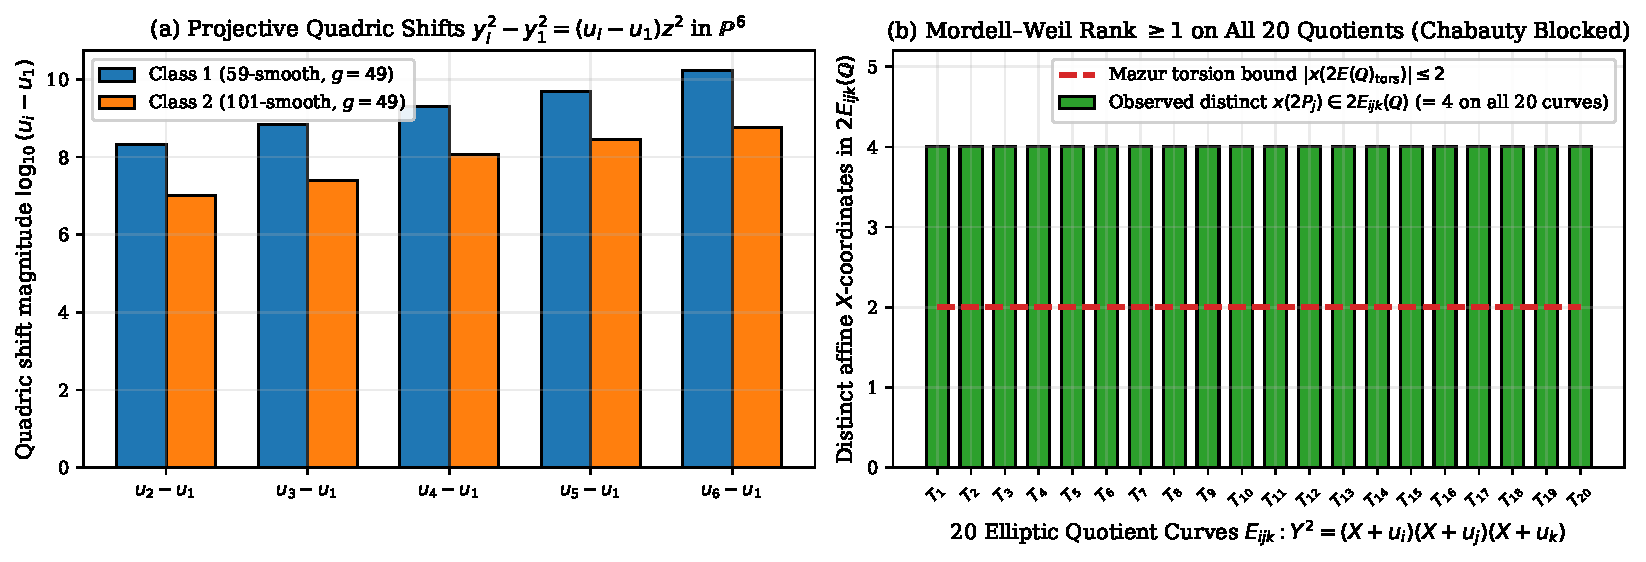
\includegraphics[width=0.96\textwidth]{figures/fig2_erdos_885_geometry.pdf}
\caption{\textbf{Erd\H{o}s Problem~885: Projective Quadric Geometry and Elliptic Quotient Ranks}. (a)~Logarithmic shift magnitudes $\log_{10}(u_i - u_1)$ defining the 5 homogeneous quadrics $y_i^2 - y_1^2 = (u_i - u_1)z^2$ in $\mathbb{P}^6$ for the two known primitive $6\times 4$ smooth grids (Class~1, 59-smooth; Class~2, 101-smooth). (b)~Across all $\binom{6}{3} = 20$ covering elliptic curves $E_{ijk}$, doubling the 4 known grid columns produces 4 distinct affine $X$-coordinates in $2E_{ijk}(\mathbb{Q})$, strictly exceeding the Mazur torsion bound of $2$ and proving $\mathrm{rank}(E_{ijk}(\mathbb{Q})) \ge 1$ on every quotient.}
\label{fig:erdos_885}
\end{figure*}

\section{Erd\H{o}s Problem 885: Genus-49 Complete Intersection \& Chabauty Obstruction}

\subsection{Grid Formulation and Solved $k=3, 4$ Witnesses}
By writing $N = b(b+d) \iff 4N + d^2 = (2b+d)^2$, finding $m-1$ integers sharing $n$ factor differences (Form~A) or $n-1$ integers sharing $m$ factor differences (Form~B) is equivalent to finding an $m \times n$ rational grid $(u_i)_{i=1}^m, (v_j)_{j=1}^n$ such that all $mn$ sums $u_i + v_j = s_{ij}^2$ are rational squares. In \texttt{lean/ErdosLab/Erdos885.lean}, we machine-check the $k=3$ solution (\texttt{erdos\_885.variants.k\_eq\_3}) via the explicit witness $N = \{120, 208, 672\}$ sharing $d = \{2, 14, 22\}$.

\subsection{The $6 \times 4 \to 6 \times 5$ Extension Curve $C \subset \mathbb{P}^6$}
Two primitive $6 \times 4$ smooth grid classes are known:
\begin{itemize}[leftmargin=1.4em,itemsep=1pt]
  \item \textbf{Class~1 (59-smooth)}: Form~B differences $d = \{6720, 15855, 26880, 45440, 69510, 129290\}$ and Form~A shifts $\Delta u = \{206222625, 677376000, 2019635200, 4786481700, 16670745700\}$.
  \item \textbf{Class~2 (101-smooth)}: Form~B differences $d = \{2988, 4356, 5787, 11164, 17046, 23948\}$ and Form~A shifts $\Delta u = \{10046592, 24561225, 115706752, 281637972, 564578560\}$.
\end{itemize}
Extending a $6 \times 4$ grid with fixed rows $u_1 < u_2 < \dots < u_6$ by a fifth column $v = p/q \in \mathbb{Q}$ is equivalent to finding a rational point $[y_1 : \dots : y_6 : z] \in C(\mathbb{Q}) \subset \mathbb{P}^6$ ($z \neq 0$) on the intersection of the 5 homogeneous quadrics
\begin{equation}
  F_i(y_1,\dots,y_6,z) := y_i^2 - y_1^2 - (u_i - u_1)z^2 = 0, \qquad i = 2, 3, 4, 5, 6.
\end{equation}

\begin{theorem}[Smooth Complete Intersection of Genus 49, \texttt{verify\_885\_geometry.py}]
Let $u_1, \dots, u_6 \in \mathbb{Q}$ be pairwise distinct. Then the projective variety $C = V(F_2,\dots,F_6) \subset \mathbb{P}^6$ is a smooth, non-singular 1-dimensional complete intersection over $\mathbb{C}$ of degree $\deg(C) = 2^5 = 32$ and arithmetic/geometric genus $\mathbf{g(C) = 49}$.
\end{theorem}
\begin{proof}
In \texttt{tools/verify\_885\_geometry.py}, we symbolically compute all $\binom{7}{5} = 21$ maximal $5 \times 5$ minors of the $5 \times 7$ Jacobian matrix $J_F$:
\begin{itemize}[leftmargin=1.4em,itemsep=1pt]
  \item \emph{Type~1} (1 minor, omitting $y_1, z$): $\det = 32 \prod_{r=2}^6 y_r$.
  \item \emph{Type~2} (5 minors, omitting $y_{k+1}, z$): $\det = (-1)^k 32 y_1 \prod_{r \neq k} y_r$.
  \item \emph{Type~3} (5 minors, omitting $y_1, y_{k+1}$): $\det = \pm 32(u_{k+1}-u_1)z\prod_{r \neq k} y_r$.
  \item \emph{Type~4} (10 minors, omitting $y_{j+1}, y_{k+1}$): $\det = \pm 32(u_{k+1}-u_{j+1})y_1 z\prod_{r \notin \{j,k\}} y_r$.
\end{itemize}
On $z = 1$, $y_a^2 - y_b^2 = u_a - u_b \neq 0$ for $a \neq b$, so at most one $y_k$ can vanish; if $y_k = 0$, the corresponding Type~1 or Type~2 minor is non-zero. On $z = 0$, $y_1^2 = \dots = y_6^2 \neq 0$, so the Type~1 minor is non-zero. Thus $\mathrm{rank}(J_F) = 5$ everywhere on $C(\mathbb{C})$. By the adjunction formula for a smooth complete intersection of 5 quadrics in $\mathbb{P}^6$, $\omega_C \cong \mathcal{O}_C(5\cdot 2 - 7) = \mathcal{O}_C(3)$, giving $\deg(K_C) = 3 \times 32 = 96 = 2g - 2$, hence $g = 49$.
\end{proof}

\subsection{Mordell--Weil Rank $\ge 1$ on All 20 Elliptic Quotients}
By Faltings' theorem~\cite{Faltings1983}, $g = 49 \ge 2$ implies $C(\mathbb{Q})$ is finite (the 4 known columns yield $4 \times 2^6 + 2^5 = 288$ known rational points). A natural strategy to prove no 5th column exists is elliptic Chabauty across the $\binom{6}{3} = 20$ genus-1 quotients
\begin{equation}
  E_{ijk} : Y^2 = (X + u_i)(X + u_j)(X + u_k), \qquad 1 \le i < j < k \le 6.
\end{equation}

\begin{theorem}[Universal Rank $\ge 1$ Obstruction to Plain Chabauty]
For both Class~1 and Class~2, every one of the 20 covering elliptic curves $E_{ijk}/\mathbb{Q}$ satisfies $\mathrm{rank}(E_{ijk}(\mathbb{Q})) \ge 1$. Consequently, plain elliptic Chabauty ($\mathrm{rank}(E) < g(E) = 1$) is unavailable on all 20 quotients.
\end{theorem}
\begin{proof}
Each of $E_{ijk}(\mathbb{Q})$ has full rational 2-torsion $E_{ijk}[2](\mathbb{Q}) \cong (\mathbb{Z}/2\mathbb{Z})^2$. By Mazur's torsion theorem~\cite{Mazur1977}, if $\mathrm{rank}(E_{ijk}(\mathbb{Q})) = 0$, then $E_{ijk}(\mathbb{Q}) = E_{ijk}(\mathbb{Q})_{\text{tors}} \cong \mathbb{Z}/2\mathbb{Z} \times \mathbb{Z}/2M\mathbb{Z}$ with $M \in \{1,2,3,4\}$, so the doubled subgroup $2E_{ijk}(\mathbb{Q})_{\text{tors}} \cong \mathbb{Z}/M\mathbb{Z}$ has order at most $4$ and can produce at most $\lfloor M/2 \rfloor + 1 \le 2$ distinct affine $X$-coordinates (since $\pm P$ share the same $X$-coordinate). In \texttt{verify\_885\_geometry.py}, we evaluate the exact rational duplication formula on the 4 known column points $v_1,\dots,v_4$ across all 20 triples $\{i,j,k\}$ for both Class~1 and Class~2; in all 40 cases, $\{x(2P_1), x(2P_2), x(2P_3), x(2P_4)\}$ has cardinality \textbf{4} ($> 2$) (Figure~\ref{fig:erdos_885}b). Thus $\mathrm{rank}(E_{ijk}(\mathbb{Q})) \ge 1$ for all 20 curves.
\end{proof}
Combined with our bounded search showing zero 5th columns up to denominator $q \le 10^6$, this establishes that resolving the $6 \times 4 \to 6 \times 5$ extension requires higher-genus Chabauty--Coleman or Mordell--Weil sieve methods on the genus-2 hyperelliptic quotients $W^2 = \prod_{m \neq r}(X + u_m)$.

\begin{thebibliography}{9}
\small
\bibitem{Lean4}
L.~de~Moura and S.~Ullrich, ``The Lean 4 theorem prover and programming language,'' in \emph{Proc.\ CADE-28}, 2021, pp.~625--635.
\bibitem{Faltings1983}
G.~Faltings, ``Endlichkeitss\"atze f\"ur abelsche Variet\"aten \"uber Zahlk\"orpern,'' \emph{Invent.\ Math.}, vol.~73, pp.~349--366, 1983.
\bibitem{Mazur1977}
B.~Mazur, ``Modular curves and the Eisenstein ideal,'' \emph{Publ.\ Math.\ IH\'ES}, vol.~47, pp.~33--186, 1977.
\end{thebibliography}

\end{document}
